\section{Calorimeter Noise simulation}
\label{sc:CaloNoise}

\begin{figure}[h!]
 \centering
 \begin{tabular}{ll}
  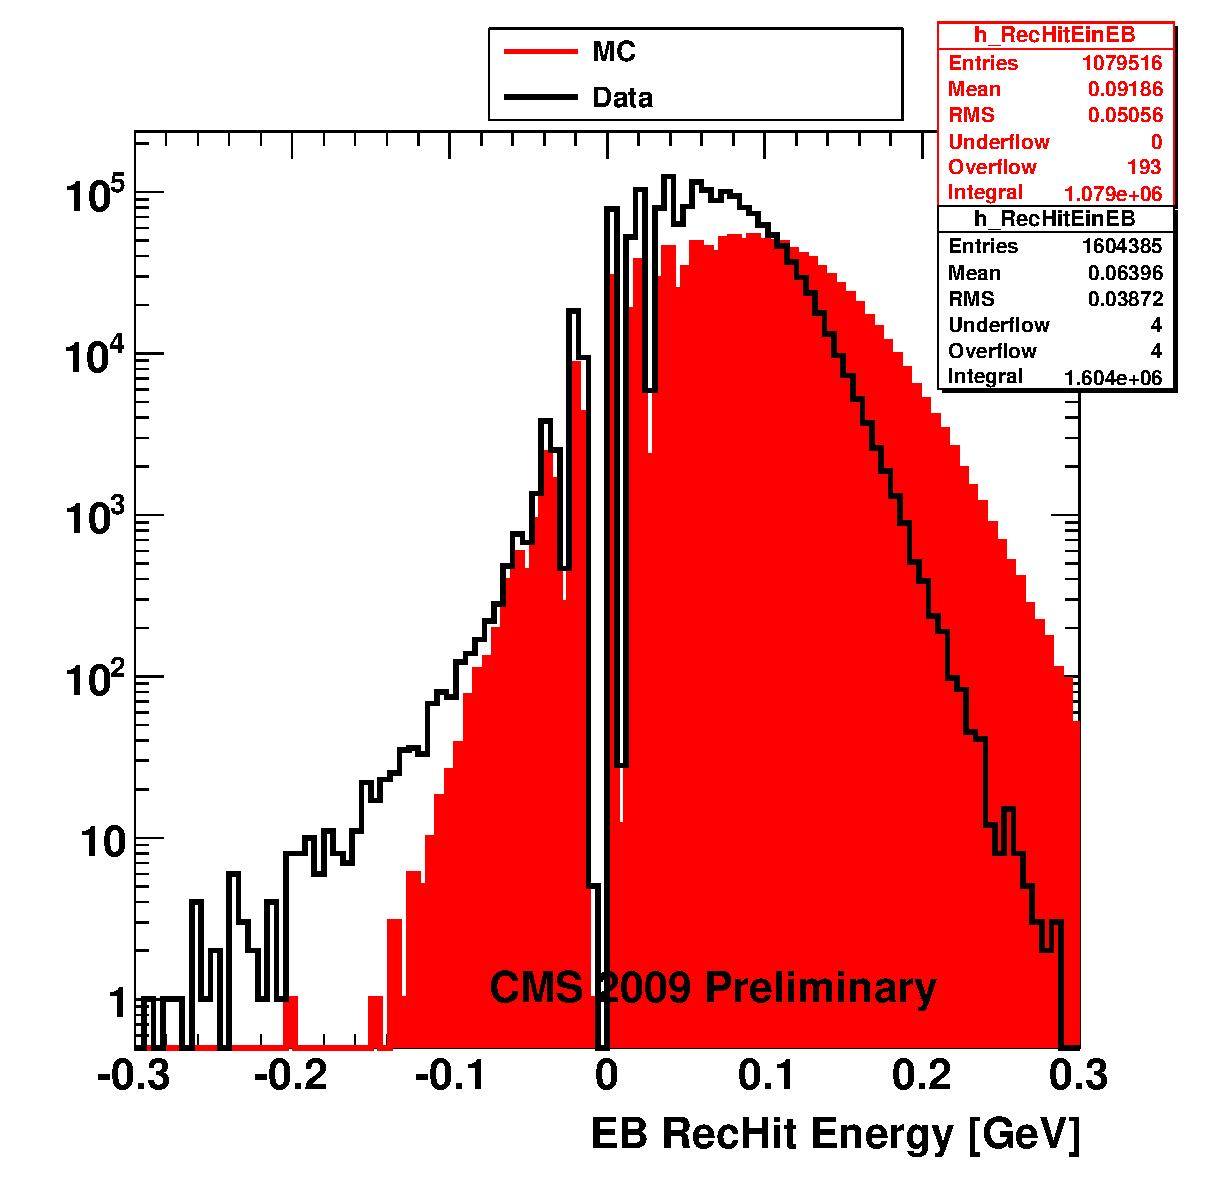
\includegraphics[width=0.33\textwidth]{plots_CaloNoise/h_RecHitEinEB.eps} &
  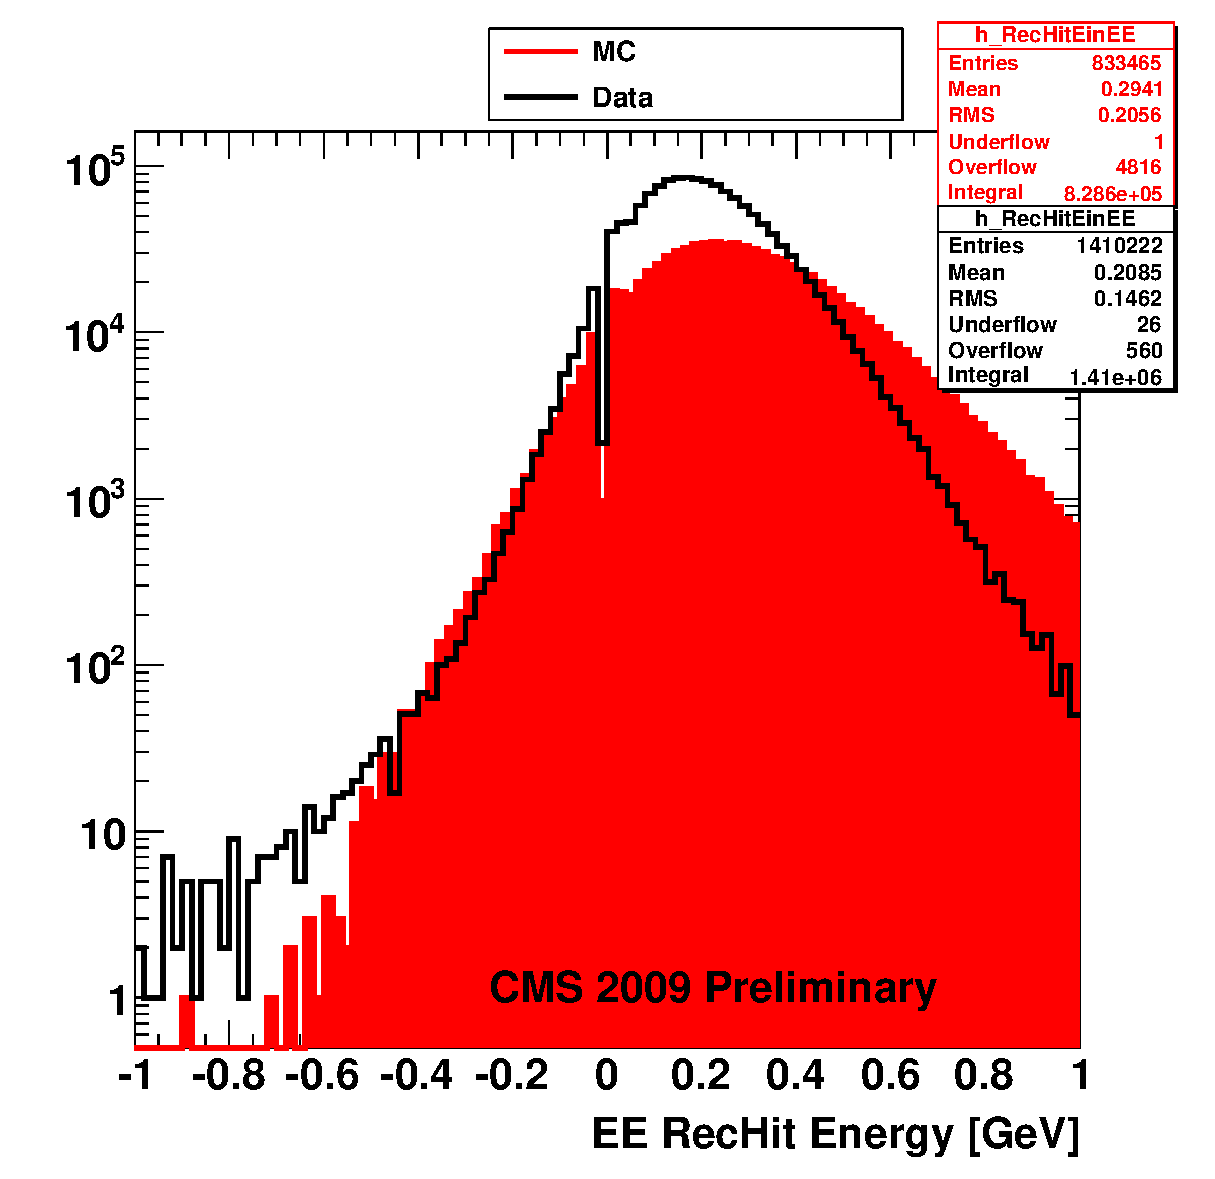
\includegraphics[width=0.33\textwidth]{plots_CaloNoise/h_RecHitEinEE.eps} \\
 \end{tabular}
 \caption{\small Comparison of the RecHit energy distributions in EB and EE for 2000 events in noise-only Monte Carlo
          and zero bias data for run 123596.\label{fig:RecHitE}}
\end{figure}

\begin{figure}[h!]
 \centering
 \begin{tabular}{lll}
  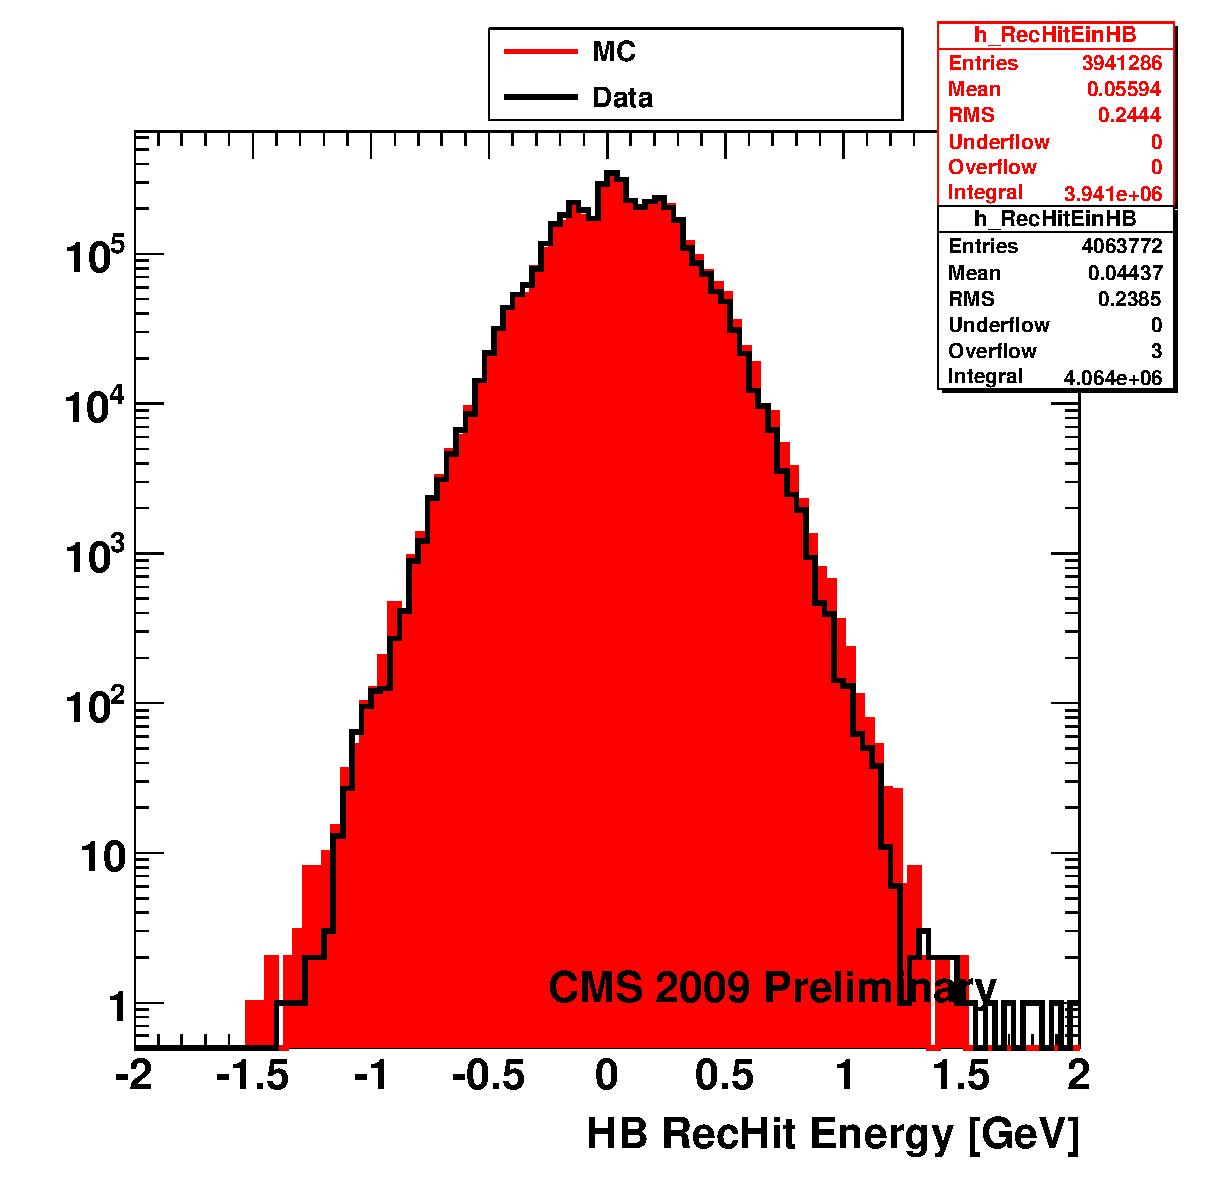
\includegraphics[width=0.33\textwidth]{plots_CaloNoise/h_RecHitEinHB.eps} &
  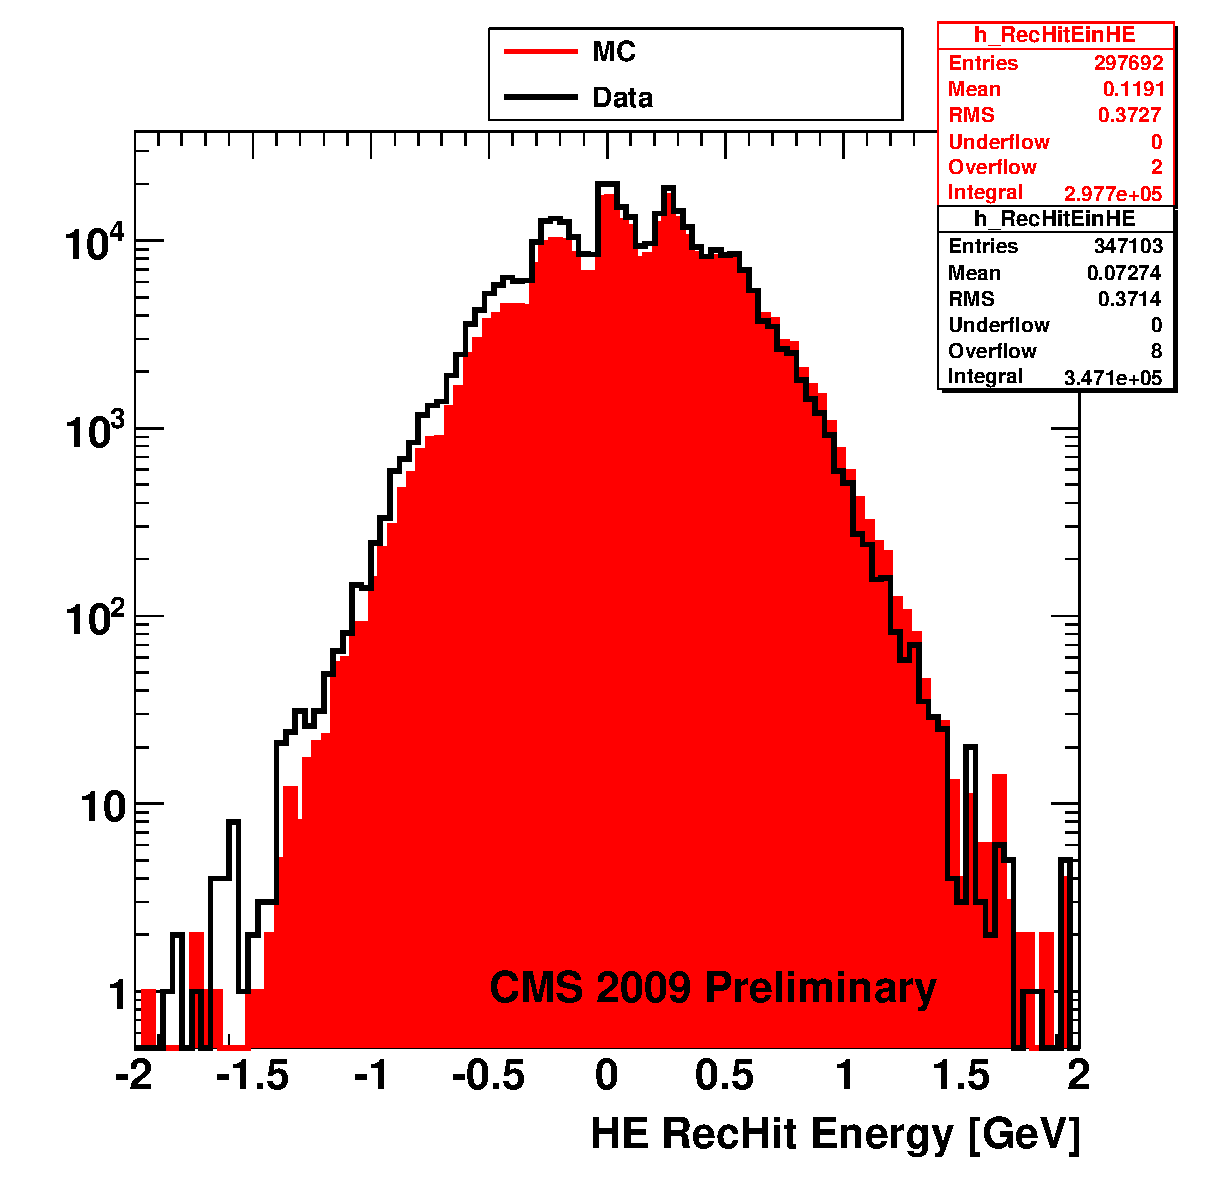
\includegraphics[width=0.33\textwidth]{plots_CaloNoise/h_RecHitEinHE.eps} &
  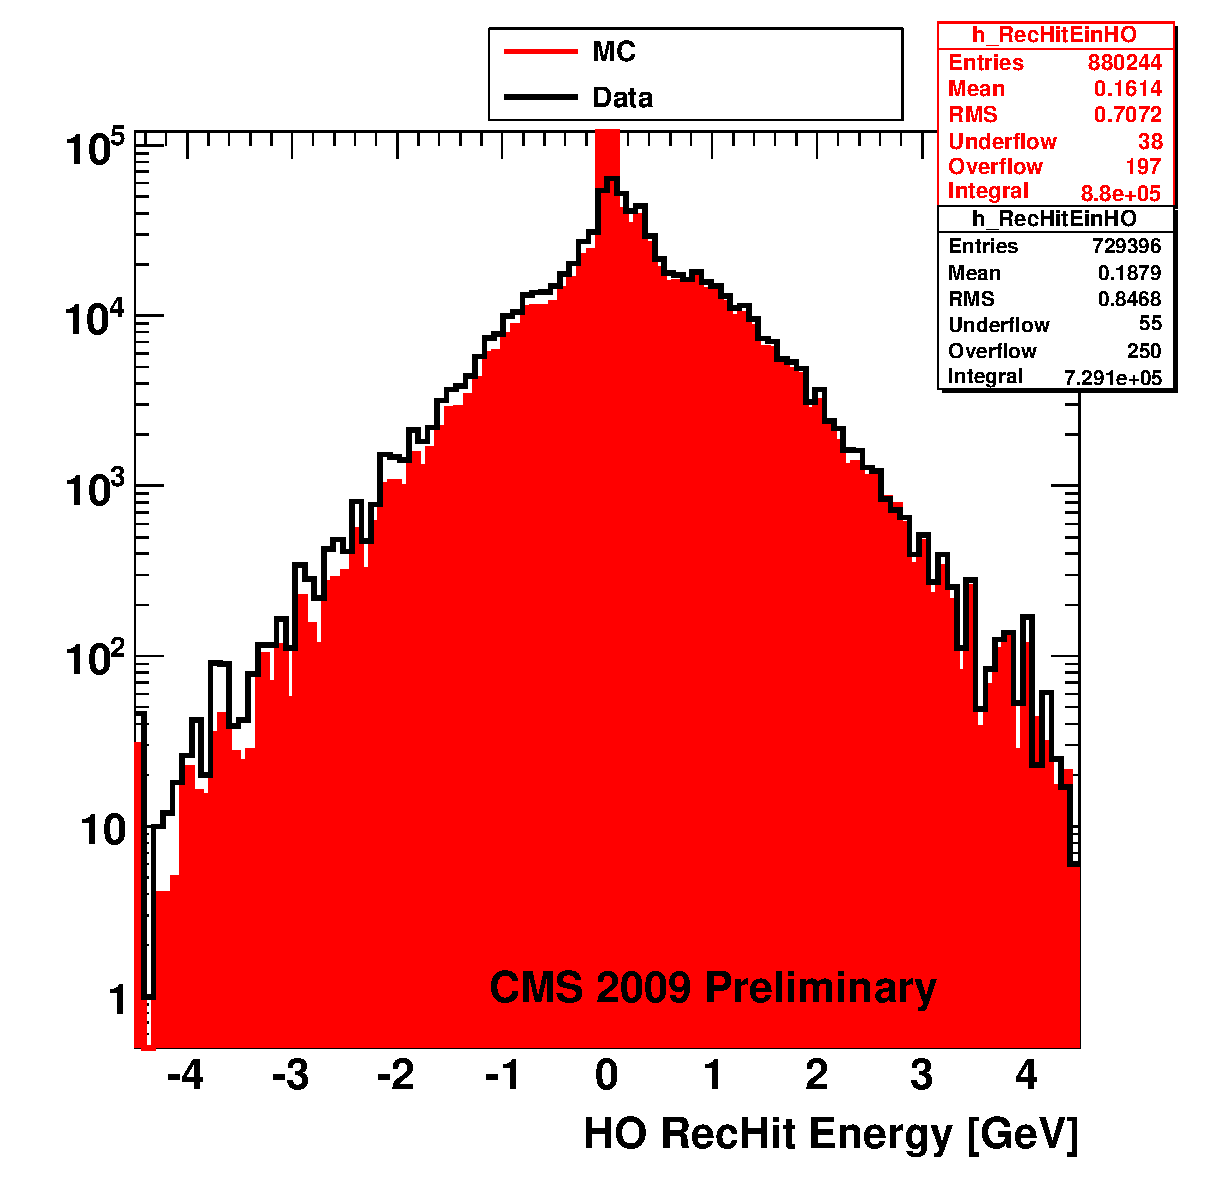
\includegraphics[width=0.33\textwidth]{plots_CaloNoise/h_RecHitEinHO.eps} \\
 \end{tabular}
 \caption{\small Comparison of the RecHit energy distributions in HB, HE, and HO for 2000 events in noise-only Monte Carlo
          and zero bias data for run 123596.\label{fig:RecHitE}}
\end{figure}

\begin{figure}[h!]
 \centering
 \begin{tabular}{ll}
  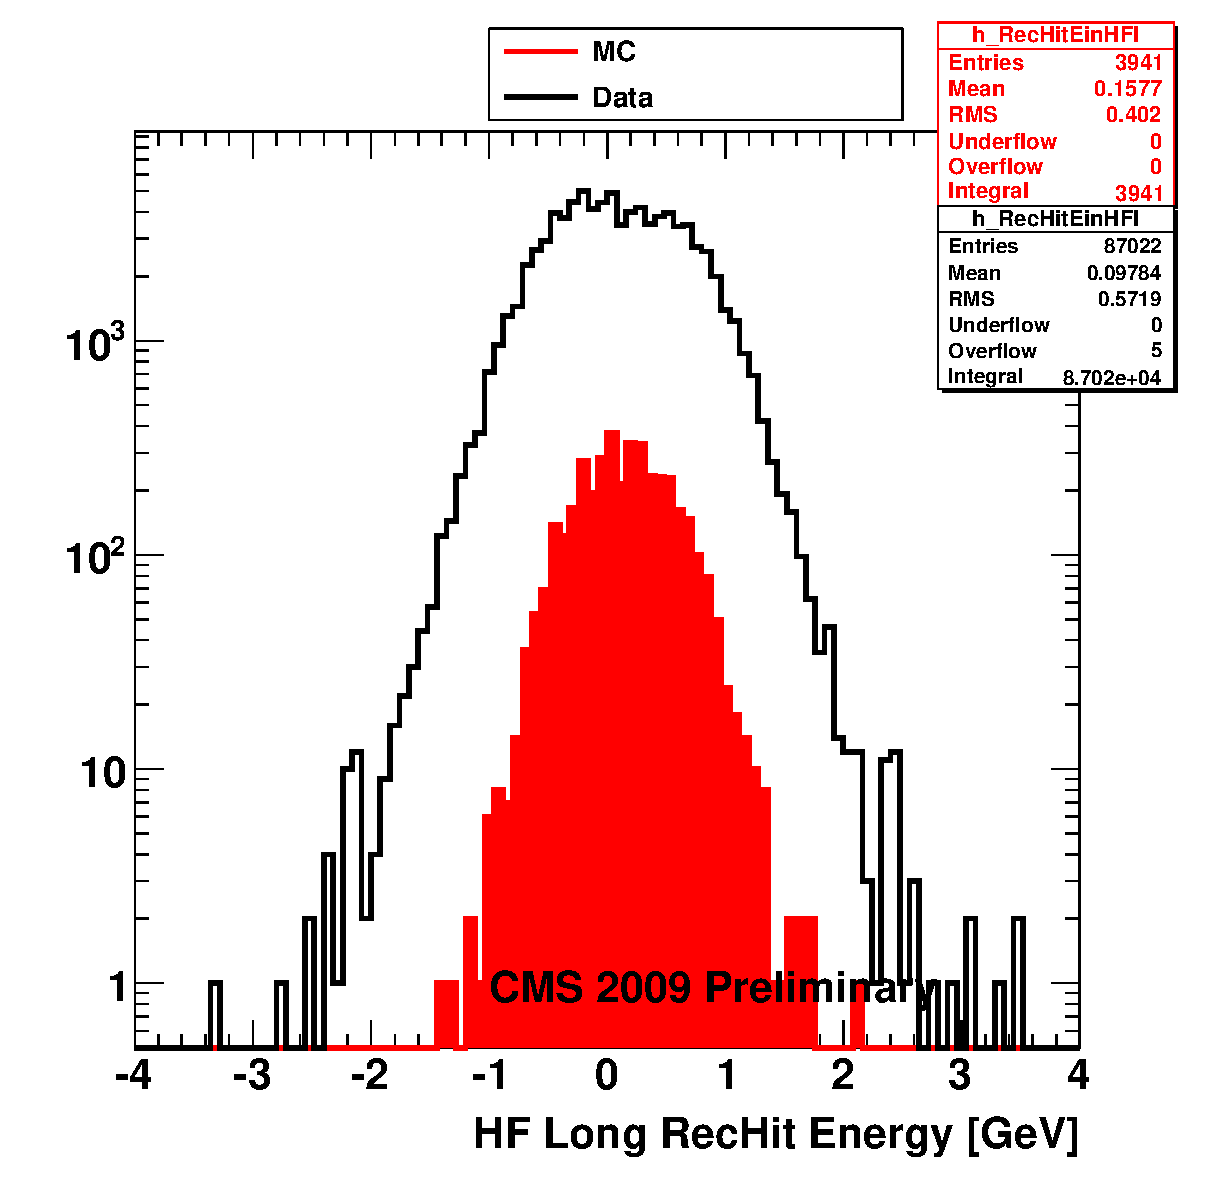
\includegraphics[width=0.33\textwidth]{plots_CaloNoise/h_RecHitEinHFl.eps} &
  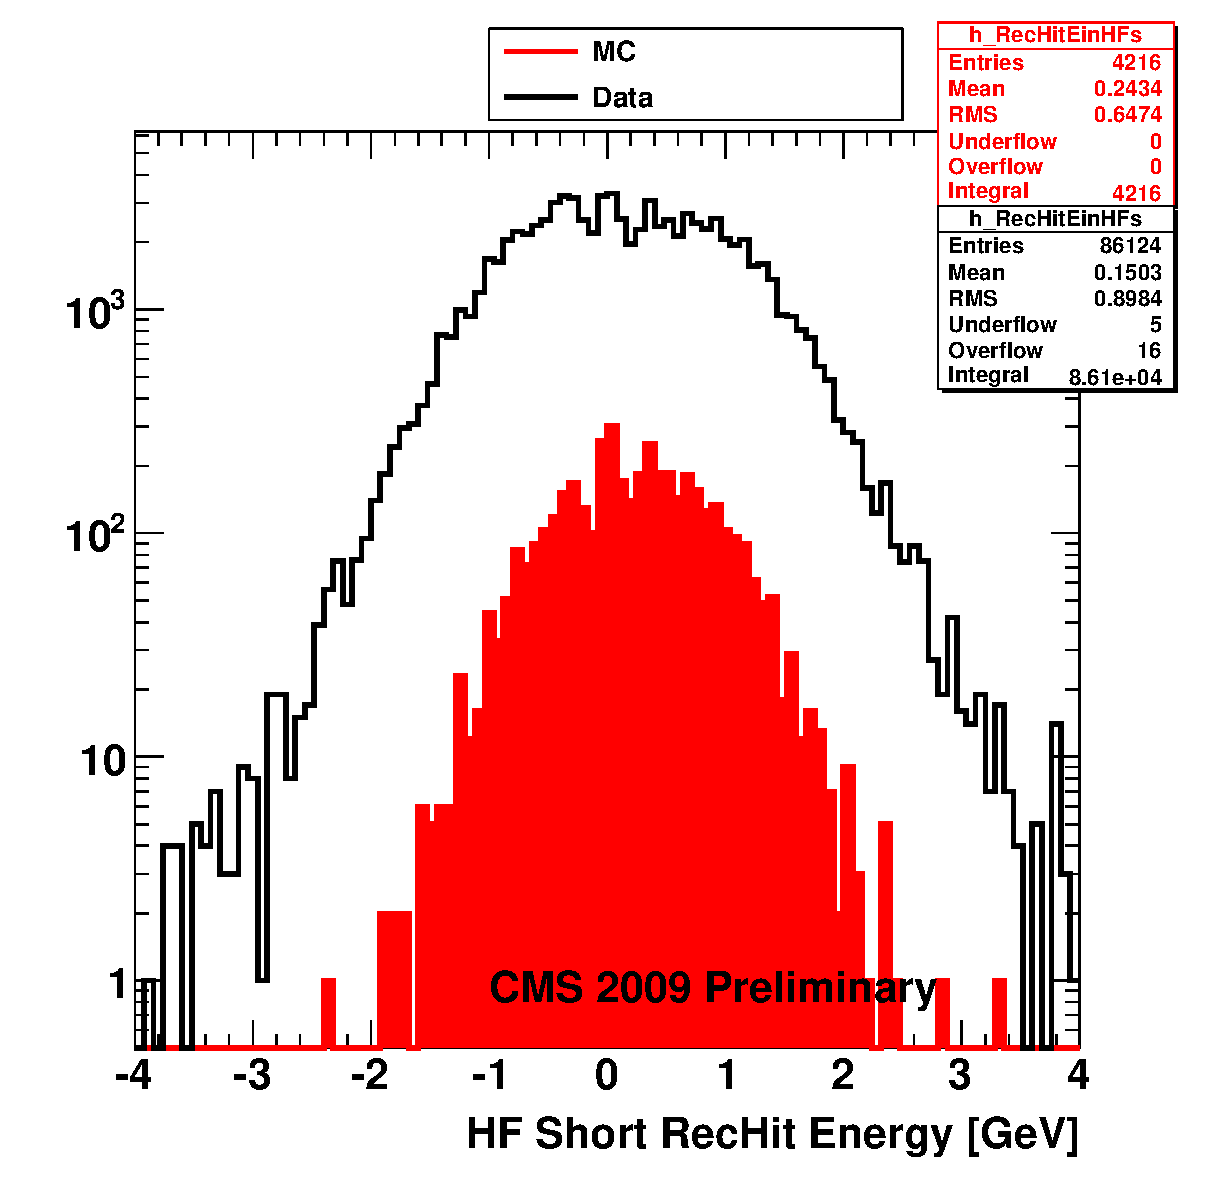
\includegraphics[width=0.33\textwidth]{plots_CaloNoise/h_RecHitEinHFs.eps} \\
 \end{tabular}
 \caption{\small Comparison of the RecHit energy distributions in HF for 2000 events in noise-only Monte Carlo
          and zero bias data for run 123596.\label{fig:RecHitE}}
\end{figure}